\section{Solution}\label{sec:solution}
\subsection{Localization}\label{subsec:solution_localization}
For the localization, a Kalman Filter (KF) or Extended Kalman Filter (EKF) \cite{b12} (according to the considered dynamic) and a distributed Weighted Least Square (WLS) has been used. In particular, each agent localizes itself running a KF/EKF that updates its prediction with only an absolute measurement (i.e. from the GPS). In a following step, each agent measures the relative distance from the others and then project them back in the world reference frame (i.e. a frame common for all the parachutes). Finally, the network runs a distributed WLS in order to share the knowledge with the team in a distributed way. The KF/EKF works as optimal filter under the hypothesis that the noise acting on the system is white, gaussian with zero mean, \textcolor{blue}{and uncorrelated from the one acting on the measurement}, the sensors are calibrated and affected by a zero mean white noise.\\
 To ensure the reaching of the average consensus the transition matrix describing the system at each time step has to be doubly stochastic, implying that the communication between agents has to be bidirectional.\\
 \textcolor{blue}{The distribution of the localization has been done applying the distribute WLS algorithm presented in the course \cite{b13}. In particular, each agent \textit{i} able to communicate with another shares its own localization and the one done on the others \textit{j} in the swarm, alongside with the associated covariance matrices. The assumption on which the algorithm is based is that the localization done by \textit{i} on agent \textit{$j_1$} is uncorrelated on the one done on \textit{$j_2$}, which implies that the covariance matrix (called C in \cite{b13}) build during the consensus is block diagonal (even though each block is not necessarily diagonal). The Metropolis-Hastings time-varying weighting scheme.\\
The result of the consensus is that each agent may have improved the localization on other that haev already seen, but also fo some furthert that were not directly measured before, and for which the information come with message exchange.}. Note that now, the self-localization of agent \textit{i} now depends also on the self localization of the others (which is embedded in the relative measurement). This implies that agent \textit{i} cannot use the output of the consensus as input of the new round of KF/EKF, because \textcolor{blue}{KFs/EKFs} cannot be used in cascade. For this reason, before running another round of localization, each agent discards the information of its position reached with the WLS and so the \textit{previous} at KF/EKF step k+1 is the output of step k. This is done to ensure that the input of a KF is uncorrelated from the output of the others.\\
In the picture, a probability of performing the GPS and the relative distance measurement are taken into account.

\subsection{Collision avoidance}
After having localized each agent, the collision avoidance is necessary to let each robot be reasonably further from the others in order to not get tangled when moving in the space. This requirement has also to be fulfilled while the agents are moving in a 3D environment, taking into account a finite size of the parachutes, the knowledge of the position of only a subset of agents (furthermore with a certain level of uncertainty). All these features may be well obtained dividing the working space with a Voronoi tessellation and enforcing each agent to move remaining inside its own cell. \\
The basic idea behind the tessellation is to assign to an agent \textit{i} all the points of the mission space $q \in \mathcal{Q} \subseteq \mathbb{R}^2$ closer to it more than to the others agents \textit{j} \cite{b1}:
\begin{equation}
    \mathcal{V}_i = \left\{ q \in \mathcal{Q} \lvert \left\lVert q-p_i \right\rVert \leq \left\lVert q-\hat{p_j} \right\rVert, \forall j \neq i, j \in \tilde{\mathcal{N}_{i}} \right\}
\end{equation}
where $p_i=\left[x_i, y_i\right]^T$ is the location of the agent \textit{i} while $\hat{p_j}$ is the one of agent \textit{j} (eventually properly projected in order to achieve some further features, as will be explained in \autoref{sec:implementation_details}).\\
The decentralization of the algorithm implies that each agent performs the tessellation of only a surrounding area of radius $R_s$, called \textit{sensing range} which is usually set at $R_s = R_c/2$, with $R_c$ the furthest distance from where an agent can measure the position of another, called \textit{communication range}. The \textit{neighbour set} $\tilde{\mathcal{N}_{i}}$ is composed by all the egents for which the position is known either by consensus or direct measure. \\
During the navigation, the entity used to represent the agent is its centroid, and so all the computations are done in order to ensure that this specific point remains inside the designed area. The finite dimension of the agent $\delta_i$ has to be taken into account because otherwise the parachute may exceed the prescribed limit even tough its centroid remains inside the cell. In order to avoid this, the dimension of the tessellation has to be shrunk such that when the centre of the agent reaches the new edge, its encumbrance arrives at the old limit. Furthermore, since the algorithm is implemented in discrete time, then the evolution of the system between one time instant and the following has to be considered beforehand, assuming that the agent may always move of the maximum amount allowed by the actuators in one time step.\\
\textcolor{blue}{Given that} the environment where the parachutes fly is a 3D space, then in principle the voronoi tessellation have to be expanded at the whole volume of movement. However, the problem can be still seen as a planar one by projecting the location of the surrounding agents in the plane of the one doing the tessellation when these are reasonably close to each others. Furthermore, in the case that the chute admits an actuation in the vertical direction, then the tessellation concept can be extended in the vertical axis in order to ensure the collision avoidance even in that dimension. Here the safe space is the one between the agents itself and a minimum height called $z_{min}$.
\subsection{High-level motion control}
\textcolor{blue}{The high-level motion control deals with the problem of how and where to move the centroid, in order to make it land on the target. Furthermore, since the centroid is a function of the single parachute location, it coordinates the agetns' movements in order to realized the prescribed centroid trajectory. The actuators command enabling this displacement are instead sintetized by the \textit{low-level controller}.}\\
In this work, the centroid is modeled as a fictional fully actuated robot with a linear dynamic in 2 dimensions, as shown in (\ref{robot}): since the target position is on the ground, the convergence in the z direction is guaranteed by the action of gravity, so the actuators must only work in the $xy$ plane.\\
\begin{equation}
    \begin{bmatrix}
        x_{i+1}\\
        y_{i+1}
    \end{bmatrix}=
    \begin{bmatrix}
        I_2
    \end{bmatrix}
    \begin{bmatrix}
        x_i\\
        y_i
    \end{bmatrix}
    +\Delta t\begin{bmatrix}
        I_2
    \end{bmatrix}
    \begin{bmatrix}
        v_{x,i}\\
        v_{y,i}
    \end{bmatrix}
    \label{robot}
\end{equation}
An LQR algorithm \cite{} has been used to find the optimal input $u$ to be fed to the \textcolor{blue}{fake agent}. This algorithm can only be used for linear systems and it finds the global optimum of the problem, which is calculated by means of a minimization of a cost function, expressed as:
\begin{equation}
    J = \sum_{k=t}^{N-1} x_k^TSx_k + u_k^TRu_k
\end{equation}
where $S$ and $R$ are the state and input cost matrices, which can be modeled to improve the state or the input minimization, and $x$ and $u$ are the actual state and input.\\
In the discrete time, finite horizon domain, the optimum input is given by:
\begin{equation}
    u_t=K_tx_t 
\end{equation}
where $K_t$ is the optimal gain matrix given by the algorithm.\\
Once the optimal control for the fictional robot is found, following the kinematics shown in the equations (\ref{robot}), its next desired position is calculated.\\
The computation of the desired position of each parachute that realize the desired movement of the global centroid is not trivial. In fact, the global centroid is a function of each parachute position, and the inverse kinematic (i.e. finding the parachutes' positions that realize a desired position in the centroid) is over-determined. \textcolor{blue}{Two solutions has been proposed to solve this problem, while a third one to be used is used in some \textit{emergency} situations to avoid collision will be presented in \autoref{sec:details_high_level}, after the motivations why it is necessary.
\subsubsection{Same control for all the chutes}
 A quick and intuitive but "forced" solution consists of feeding in the parachutes the exact same control input found in the LQR problem since if every parachute moves in the same way then the global centroid will be moved accordingly.
 \subsubsection{Inverse kinematics}
  A more robust solution comes from comparing this problem to the well-known and solved problem of redendancy in robotics. In fact, as in overactuated manipulators there are infinite joints' position realizing a desired end effector position, here infinite agents' positoin realize the centroid one. However, a numerical approach has been developed in the past years to solve inverse kinematics by a \textit{postural task}, which is just an arbitrary chosen secondary task in the joint space that does not affect the motion of the end-effector  but identifies one solution among the infinite ones \cite{b5} \cite{b6}.\\
In this specific case two possible secondary tasks may be to let each single agent converge toward the land target or toward the global centroid. The algorithm can give more priority to pricipal or secondary requirement  according to a weighting value that can be chosen arbitrary.}

\subsection{Low-level motion control}
Given the single parachute target point from the high-level control, the goal of the low level control is to provide the input that ensures to move towards it while not exceed the motion boundaries identified by the Voronoi tessellation. 
\subsubsection{Control of linear model}
In case of linear dynamics, one possible control law is the one proposed by \cite{b1}:
\begin{gather}
    \label{eq:proportional}
    u=-k_p\left(p_i - C_{\mathcal{V}_i}\right)\\
    \label{centroid}
    C_{\mathcal{V}_i} = \frac{1}{M_{\mathcal{V}_i}}\int_{\mathcal{V}_i}\varphi\left(q\right)qdq \text{ , } M_{\mathcal{V}_i} = \int_{\mathcal{V}_i}\varphi\left(q\right)dq
\end{gather}
with, for the planar motion, $\varphi\left(q\right)$ is a bivariate pdf centred in the point identified by the high level control. \textcolor{blue}{This controrl law uses the property that each point inside the voronoi cell can be reached by the agent with a staright motion}.\\
For what concerns the control on the vertical axis, as said before the velocity input has to be constrained. In particular, a proportional gain has been chosen to break when the $z_{min}$ is near to the parachute:
\begin{equation}
\label{control_law_z}
    \begin{gathered}
        k_{pz}=-\bar{v}_z/R_{sv}\\
        u_{tmp}=-\bar{v}_z-k_{pz}(z_i-z_{min,i})\\
        v_z=\min(u_{tmp}, v_{z,min}-\bar{v}_z)
    \end{gathered}
\end{equation}
In this way, when there is non parachute under the agent $i$, $(z_i-z_{min,i})=R_{sv}$ and so the control $v_z$ is zero, meaning that there is no need to break. On the other hand, when $(z_i-z_{min,i})=0$, meaning that the parachute would not want to go down because the other agents is too near, the input is $v_{z,min}-\bar{v}_z$, such that when in the dynamics it is added the effect of gravity (\ref{eq:model_1},\ref{eq:NL}) the sum results in the minimum vertical velocity: the agent cannot stop in the air but has to descent with some velocity.\\
The physical actuation in z opens or closes the sails, meaning that it changes the the $\beta$ coefficient in (\ref{eq:drag_force}) and so the free falling velocity. It has been decided to considered $\beta$ as constant and we have directly modified the velocity.\\
\textcolor{blue}{Since the external disturbances act directly on the positions, then the effective velocities can be locally grater or smaller than the boundaries.}
\subsubsection{Contorl of the unicycle model}
\textcolor{blue}{Since the trajectory followed by the nonlinear agents may exceed the voronoi cell limits with the afermentioned control law, a more complex one has to be used. In this work, the control law (\ref{eq:control_law}), proposed by \cite{b4} is allows to guarantee the convergence of the parachute towards the target in a fast and elegant way (without the use of a PID controller), and also to find the so called \textit{Feedback Motion Predict}, which is the area that can be occupied by the parachute during the execution of the control law (\ref{eq:control_law}).}
\begin{equation}
\label{eq:control_law}
    \begin{gathered}
        v_y = k_v\max\Big(0,\begin{bmatrix}
           \cos{\theta} & \sin{\theta}
       \end{bmatrix}(C_{\mathcal{V}_i} -p_i)\Big)\\
        \omega = k_{\omega}\atantwo\Big(\begin{bmatrix}
           -\sin{\theta} \\ \cos{\theta}
       \end{bmatrix}^T(C_{\mathcal{V}_i} -p_i),\begin{bmatrix}
           \cos{\theta} \\ \sin{\theta}
       \end{bmatrix}^T(C_{\mathcal{V}_i} -p_i)\Big)
    \end{gathered}
\end{equation}
\begin{figure}[t]
    \centering
    \subfloat[][\emph{Truncated Ice-Cream Motion Cone updating as the agent moves.}]{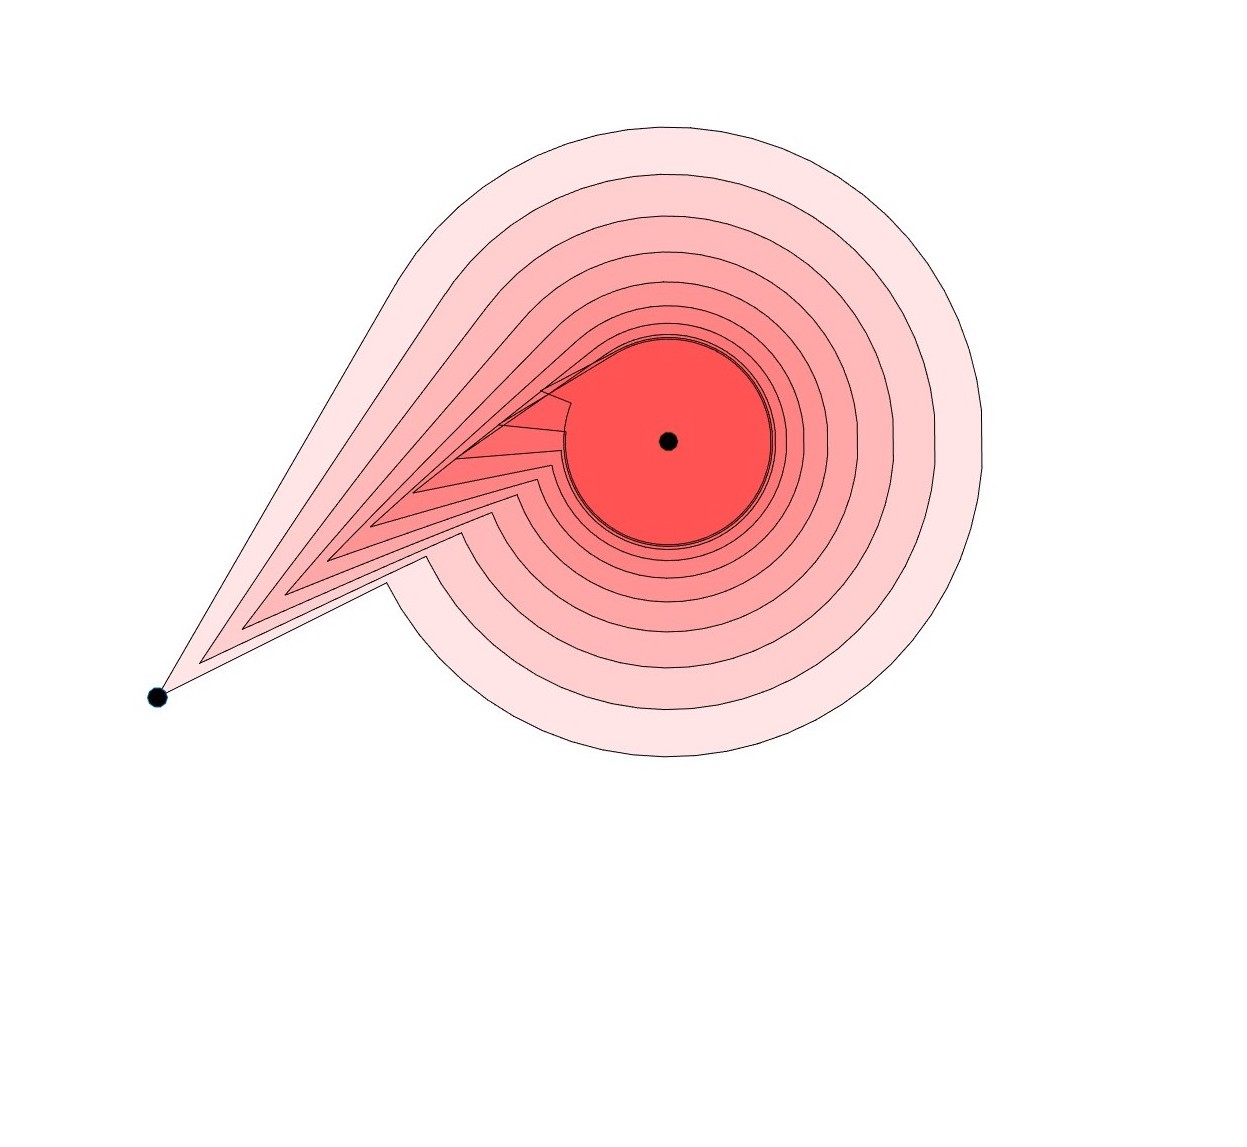
\includegraphics[scale=.08]{images/cone.jpg}} \quad
    \subfloat[][\emph{The cone is moved to be fit into the Voronoi cell.}]{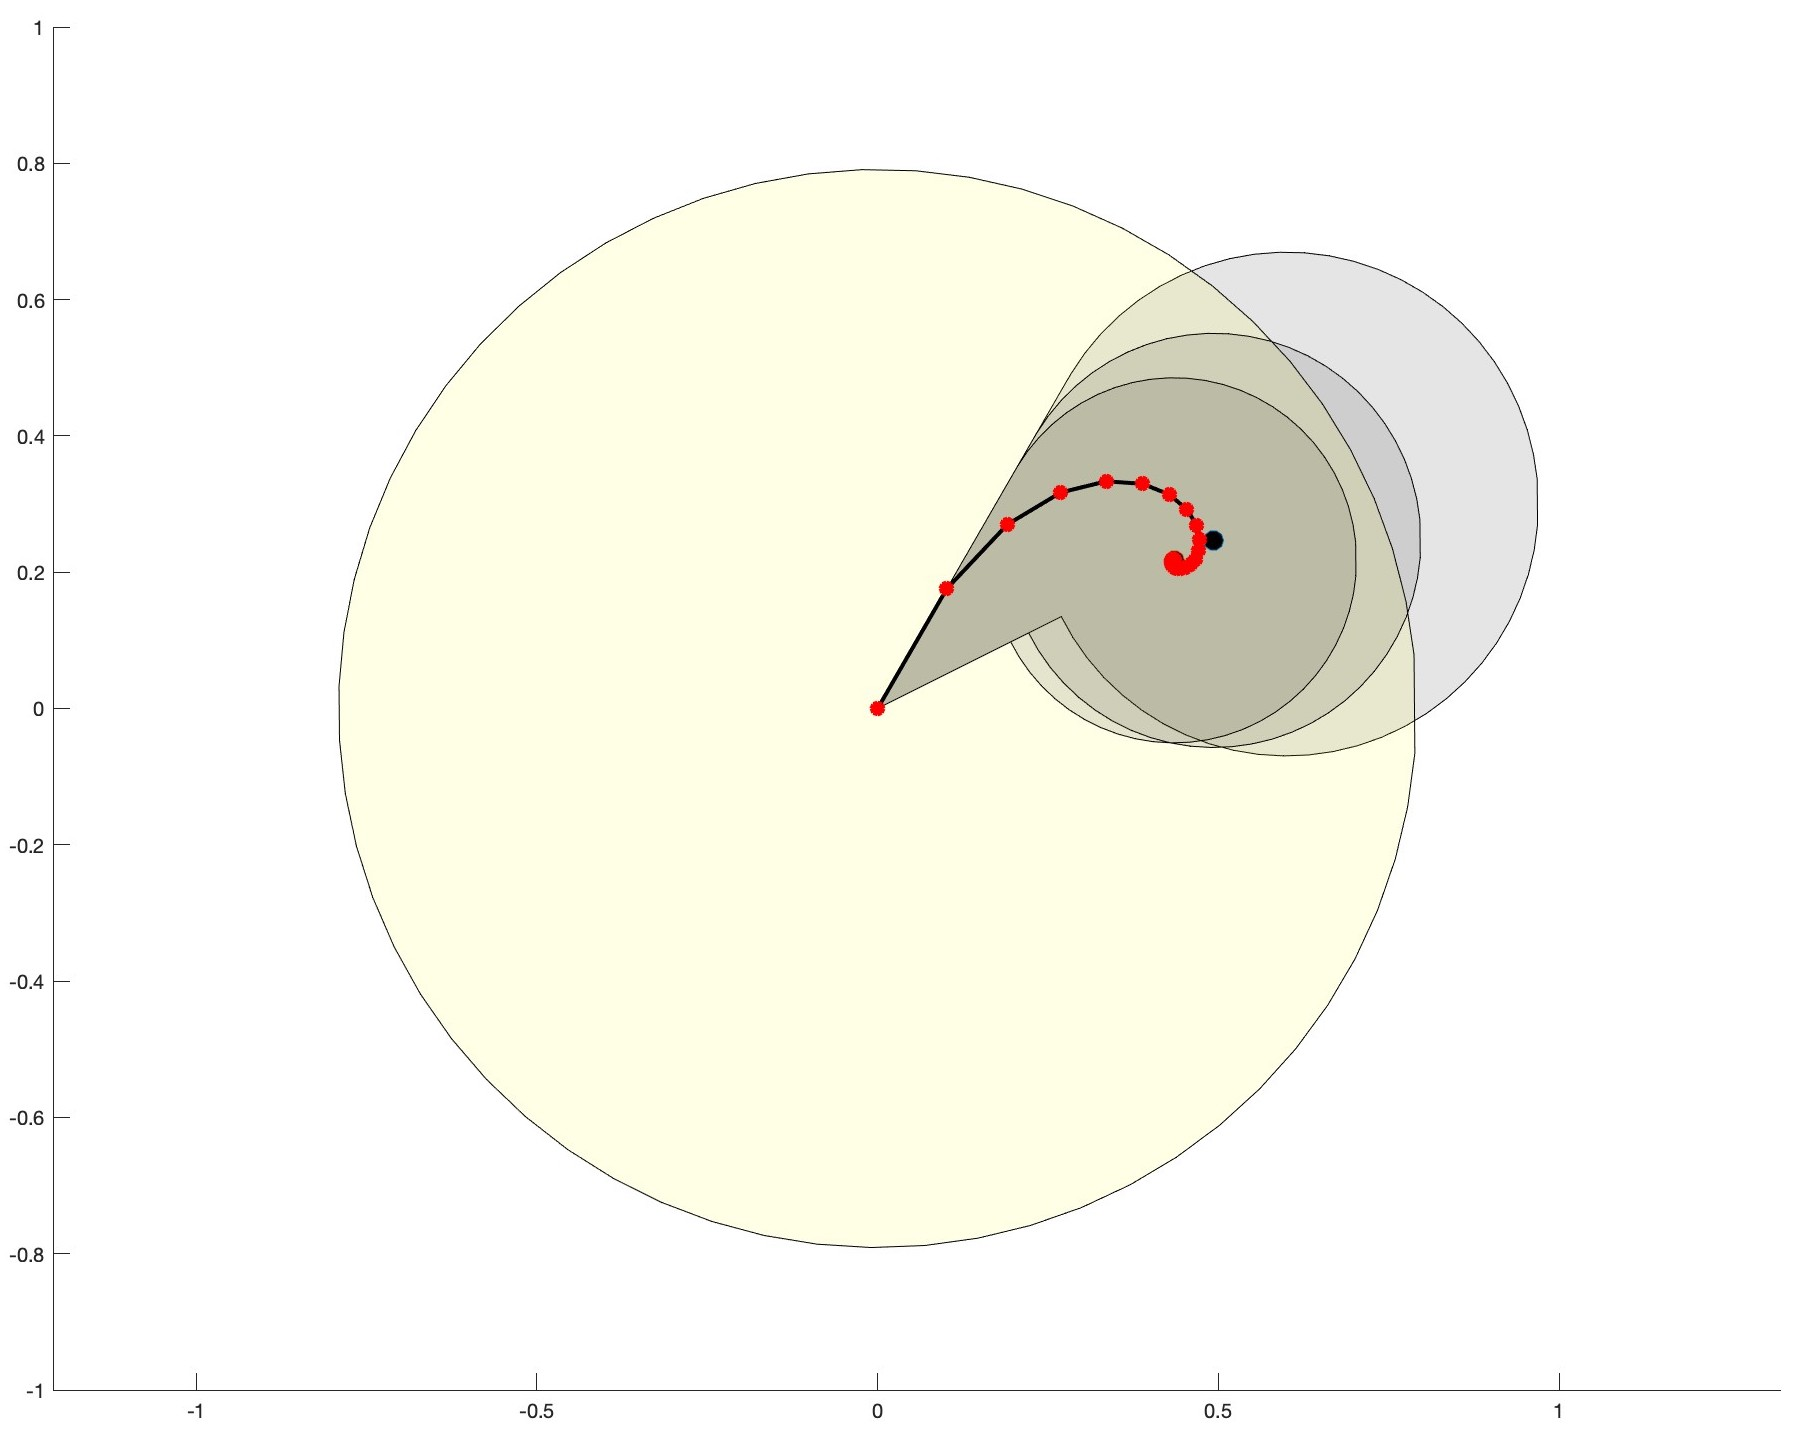
\includegraphics[scale=.07]{images/mot_pred.jpg}}
    \caption{Feedback Motion Prediction area for non-linear dynamics.}
    \label{fig:motion_pred}
\end{figure}

As already mentioned in the section \ref{unicyle}, the forward velocity is saturated to be at minimum zero, so that the parachute can never move backward but it is not forced to move at a minimum velocity in any case as happen in the real chutes. This assumption simplifies the control, becasue in the case of non-zero positive minimum velocity, \textcolor{blue}{and at least with this controlp policy} there is no guarantee that the parachute will not exit the Voronoi cell, for example when it is too close to the boundary.\\
\textcolor{blue}{To make sure that the parachute will not violate the Voronoi cell boundary, the FMP is initially calculated and, if it exits the cell, the arrival point (i.e. the new centroid founded by (\ref{centroid})), is moved closer to the actual position of parachute iteratively until the FMP fits into the Voronoi cell (as could be seen in \autoref{fig:motion_pred}).\\
\cite{b4} proposed differnt wais to define valid FMP areas, and among them it is chosen the \textit{Truncated Ice-Cream Motion Cone}, because it is the less conservative but smaller.}